\documentclass[twocolumn]{article}

\usepackage{hyperref}
\usepackage{graphicx}
\usepackage{../../usenix-2020-09}

\bibliographystyle{ieeetr}

\microtypecontext{spacing=nonfrench}

\title{Automatically Propagating Resources to Avoid~Data~Loss in Distributed~Filesystems}
\author{John Cesarz \& Shreyas Minocha}

\begin{document}

\maketitle

\section{Introduction}

There is often a need to publicly archive valuable data in a manner that is resistant to accidental data loss, owing to either system failure or maintainer neglect.\cite{shi-2019}
A common approach to sharing data within a community with redundancy is to use peer-to-peer networks like BitTorrent, which served over 7 million downloads in 2008.\cite{zhang-2011}
However, BitTorrent-based file sharing suffers from risks of data loss when the number of peers sharing a torrent is low.
BitTorrent has no mechanism for triggering the replication of ``at-risk files'', instead relying on the users of the network to coordinate this.
However, in practice, at-risk files are often neglected, until the last few peers sharing the file disappear, at which point the file is lost.\cite{zhang-2011}
Another more recent peer-to-peer technology is IPFS\cite{trautwein-2022}, but IPFS doesn't have in-network mechanisms for handling resource disappearance either.
Our goal is to find ways to find ways to prevent the problem of data loss in peer-to-peer file sharing networks by cleverly triggering replication of at-risk files.
We built a prototype of a distributed, content-addressable file system.
We evaluated our solution on the basis of its efficiency at transferring files over the network and at its memory overhead.
Our prototype comes with a practical, user-friendly interface: the ability to mount the distributed file system as a file system directory.
It also supports the assignment of user-friendly filenames of files within directories.

\section{Background}

We designed our distributed filesystem with archival use in mind.
In such systems, new data is frequently added, but existing data is rarely modified or deleted.
For archival systems, data generally needs to be stored for long periods of time—much longer than the lifetime of the typical disk.
As a result, redundant copies of data need to be maintained in order to support data integrity in the event that a single disk fails.

Making a filesystem distributed also introduces several unique problems.
Potential consumers of a particular piece of data need to be able to determine which nodes in the network contain that data and request it.
The lack of a central node also complicates the process for maintaining redundancy in the event of a node's failure.

\section{Methods}

\subsection{Content-Addressed Storage}\label{sec:cas}

We use a Merkle tree~\cite{merkle-1982} to represent the filesystem hierarchy.
We split file content into ``chunks''—pieces of data up to 4 MiB long.
Each file is represented as an ordered sequence of chunks.
Each directory is represented as an ordered sequence of name-object pairs, where the object is the identifier for either a file or a directory.
We consider files, directories, and chunks to be \textit{resources}.
Every resource is uniquely identified as an \textit{object}, which is a SHA256 hash of a unique, deterministic serialization of a resource.
At present, resources are serialized to JSON, but future versions may switch to more efficient formats like protobuf.
At the moment, all resources on the filesystem are stored in-memory; in the future this will likely be changed so that resources are stored persistently on a backing filesystem.
To work around this limitation of our current prototype, applications may use memory-backed files.

\subsection{Networking}

At present, the filesystem allows manually specifying peers by their network addresses on the command line.
When a peer $X$ successfully connects to another peer $Y$, $Y$ also automatically connects to $X$ and tracks it as one of its peers.
When a peer $X$ attempts to access a resource that it does not have access to locally, it attempts to fetch it from one of its peers.
Upon successfully finding a resource by querying another peer, peer $X$ caches said resource, saving a local copy.
At the moment, networking uses a packet abstraction built on top of TCP, in order to avoid needing to reassemble resources larger than the maximum UDP packet size.
Future versions may use a UDP-based system instead in order to improve performance.

\subsection{Interface}

Our distributed filesystem is implemented in userspace using FUSE, in order to facilitate ease of testing.
Our implementation is written in the Rust programming language in order to take advantage of its memory safety and concurrency guarantees.
The filesystem is organized in such a way that any resource can be accessed directly by SHA256 hash.
For example, an object whose hash is \texttt{aaa\dots aaa} can be accessed at \texttt{/path/to/mountpoint/aaa\dots aaa}.
Entries in a directory can also be accessed by name.
For example, if \texttt{aaa\dots aaa} is a directory containing a file named ``myfile'', ``myfile'' can be accessed at \texttt{/path/to/mountpoint/aaa\dots aaa/myfile}.
The FUSE mount is read-only, because modifying a file or directory would result in the hash of that resource changing.
As a result, a set of directories to be added to the filesystem must be specified using a compile-time flag.
% todo: mention something about how it would eventually be good to allow files/peers to be added after start

\section{Evaluation}

\subsection{Memory Usage}

As mentioned in Section~\ref{sec:cas}, our prototype currently stores file data in memory.
However, we include some measurements of our memory use for the sake of completeness.

We used a test dataset consisting a total of 1116 files, totalling 192 MB.\@
Ten of these files were nested within directories at a depth of 10.
The dataset contained a variety of file sizes, with 1010 100-byte files, 100 100 KB files, and 6 files ranging in size from 1 MB to 100 MB.
Each file was filled with randomly generated binary data.
Transferring this dataset using our prototype used 231 MB of memory and took 323.85 seconds.
When transferring the same data using IPFS, the client process used 67 MB of memory and took 68.32 seconds.

\subsection{Transfer Speed}

We evaluated our prototype's file transfer speeds on files with various sizes.
Each file was filled with randomly generated binary data.
All 9 files were added to a directory, which was then added to the filesystem.
When measuring the speed of our prototype, each file was requested by name under its parent directory, which was referenced by hash.
When measuring the speed of IPFS, each file was requested by CID.\@
Figure~\ref{fig:speed} shows the transfer speeds achieved by our prototype (``DFS'') and IPFS for single files with sizes ranging from 1 MB to 500 MB.\@

\begin{figure}\label{fig:speed}
	\caption{Data transfer speed as compared with IPFS's data transfer speed}

	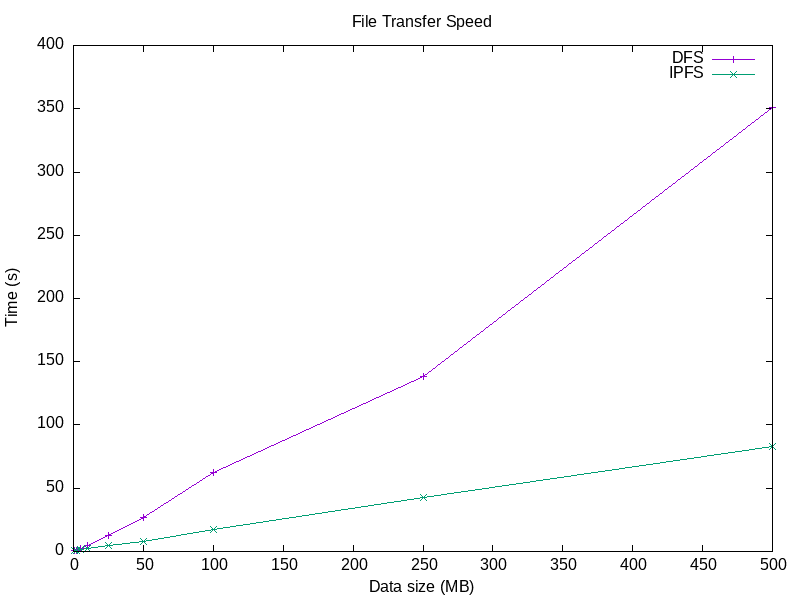
\includegraphics[width=\columnwidth]{data/speed.png}
\end{figure}

\section{Future Work}

\subsection{Peer Discovery}

One important next step is to implement automatic peer discovery.
For this, we will use a distributed hash table (DHT), similar to existing systems.
For instance, BitTorrent uses a variant of Kademlia~\cite{maymounkov-2002}.
We could also use the DHT from Pastry~\cite{rowstron-2001}, together with its overlay and routing networking.
Finally, Chord~\cite{stoica-2001}could also be an option for the DHT we use to enable peer discovery.
We will conduct an evaluation of the strengths and weaknesses of these tools for our application to make this choice.

\subsection{Resource Peer Tracking}

To efficiently detect resources that have a low number of peers, we will assign, to each resource, a peer responsible for tracking all peers that have that resource (``tracker peer'').
When this number drops below a threshold, which we term the \textit{replication threshold}, the tracker peer will attempt to trigger network-wide replication of the resource.
When the tracker peer for some resource itself goes offline, the DHT will pick a new tracker node for the resource.
Our system will determine the replication threshold based on heuristics that account for the size of the resource, the number of peers in the network, and the number of peers that have the resource.

Upon implementing a self-bootstrapping peer discovery process using a DHT, we will benchmark peer discovery times over a variety of network topologies.
We will use graph structures modelled off of large scale networks like the world-wide web to simulate typical applications of our technology.
We will evaluate our system by running it on a network of peers, and simulate peer loss.
We will use BitTorrent and IPFS as baselines for comparison.

\section{Conclusion}

We successfully built a prototype of a content-addressed file system with mechanisms for requesting and sharing files over the network.
We also built a filesystem layer that allows users to try our prototype with ease.
Our artifacts are available in our \href{https://github.com/shreyasminocha/comp517-project/tree/master/project/dfs}{repository}.

\bibliography{report}

\end{document}
